\documentclass[12pt,a4paper]{article}
\usepackage[dvipsnames]{xcolor}
\usepackage[utf8]{inputenc}
\usepackage{amsmath}
\usepackage{mathtools}
\usepackage{marvosym}
\usepackage{wrapfig}
\usepackage{hyperref}
\usepackage{float}
\usepackage{multicol}
\hypersetup{colorlinks,citecolor=black,filecolor=black,linkcolor=black,urlcolor=black}
\usepackage{pdfpages}
\usepackage{amsfonts}
\usepackage{amssymb}
\usepackage{fancyhdr}
\usepackage{chemfig}
\usepackage{graphicx}
\usepackage[T1]{fontenc}
\usepackage[magyar]{babel}
\usepackage{bm}
\usepackage{tikz, tcolorbox}
\usetikzlibrary{positioning}
\usepackage{verbatim}
\usepackage{amsmath,esint}
\usepackage{setspace}
\usepackage{qtree}
\usepackage{multido}
\usepackage{mathptmx} % Times New Roman betűtípus
\usepackage{listings}

\lstset{
    language=Matlab,
    inputencoding=utf8,
    extendedchars=true,
    basicstyle=\ttfamily\small,
    frame=single,
    breaklines=true,
    numbers=left,
    numberstyle=\tiny,
    literate=
        {á}{{\'a}}1
        {é}{{\'e}}1
        {í}{{\'i}}1
        {ó}{{\'o}}1
        {ö}{{\"o}}1
        {ő}{{\H{o}}}1
        {ú}{{\'u}}1
        {ü}{{\"u}}1
        {ű}{{\H{u}}}1
        {Á}{{\'A}}1
        {É}{{\'E}}1
        {Í}{{\'I}}1
        {Ó}{{\'O}}1
        {Ö}{{\"O}}1
        {Ő}{{\H{O}}}1
        {Ú}{{\'U}}1
        {Ü}{{\"U}}1
        {Ű}{{\H{U}}}1
}
\renewcommand{\figureautorefname}{ábra}
\newcommand{\abrara}[1]{\hyperref[#1]{\ref*{#1}.~ábra}}
\newcommand{\Pointilles}[1]{%
\par\nobreak
\noindent\rule{0pt}{1.5\baselineskip}% Provides a larger gap between the
\multido{}{#1}{\noindent\makebox[\linewidth]{\dotfill}\endgraf}
\bigskip% Gap between dots and next paragraph
}
\newcommand{\feladat}[1]{%
\phantomsection
\subsection*{#1. feladat}%
\addcontentsline{toc}{subsection}{#1. feladat}%
}
\usepackage{pgfplots}
\pgfplotsset{height = 10cm, width=15cm,compat=1.9}
\usepackage[left=2cm,right=2cm,top=2cm,bottom=2cm]{geometry}
\setlength{\parindent}{0pt}
\setlength{\parskip}{0em}
\pagestyle{fancy}
\fancyhf{}
\cfoot{\thepage. oldal}

% Másfeles sorköz beállítása
\onehalfspacing

\begin{document}

\begin{titlepage}
\centering


\includegraphics[width=.8\textwidth]{bme_logo_nagy.jpg}

\vspace{1em}

{
\large
BUDAPESTI MŰSZAKI ÉS GAZDASÁGTUDOMÁNYI EGYETEM\\ VILLAMOSMÉRNÖKI ÉS INFORMATIKAI KAR\\ MESTERSÉGES INTELLIGENCIA ÉS RENDSZERTERVEZÉS TANSZÉK
}

\vspace{6em}

{
\Huge
\textbf{Rezgésanalízis}
}

\vspace{3em}

{
\huge
Intelligens beágyazott rendszerek laboratórium\\

\vspace{.2em}

\large
(BMEVIMIMA21)
}

\vspace{9em}

{
\Large
\textit{Készítette:}\\
\vspace{.5em}
\textbf{Pál Patrik, Gavallér Dávid}\\
\vspace{.5em}
\textbf{AIQTQW, ES02RO}
}

\vspace{12em}

{
\large
BUDAPEST, \today
}
\end{titlepage}

\tableofcontents

\newpage

\section{Bevezetés}

\subsection*{A mérés célja}
A mérés során egy piezoelektromos gyorsulásérzékelő segítségével rögzítjük egy ventilátor, illetve egy hangsugárzóval gerjesztett mechanikai rendszer rezgéseit, az Audacity program segítségével, majd MATLAB környezetben elemezzük ezeket. Ezek a mérések és elemzések valódi ipari felhasználások során lehetővé teszik a rezgő mechanikai rendszerek vizsgálatát, lehetővé téve így a hibák gyorsabb felismerését és adott esetben megelőzését.

%kell?
%A mérés során állandósult és változó frekvenciájú jelek spektrumát, továbbá egy mechanikai rendszer amplitúdómenetét vizsgáljuk. A feladatok között szerepel a ventilátor rezgésének elemzése, az aszinkron motor fordulatszám-változásának és slipjének meghatározása, valamint egy káros mechanikai jelenség felismerésére alkalmas mérési módszer kidolgozása. Kiegészítő feladatként egy csengőhang főbb spektrális komponenseit és lecsengését is meghatározzuk, majd a mért eredmények alapján a hangot újra előállítjuk.

%Írhhatjuk még az általános adatokat a műszerekről

\subsection*{A méréshez használt eszközök}
\begin{itemize}
	\item Piezoelektromos gyorsulásérzékelő
	\item Töltéserősítő
	\item Oszcilloszkóp
	\item Számítógép
\end{itemize}

\newpage

\section{Mérési feladatok}

\feladat{1}

\subsubsection*{Feladat leírása}

Helyezze el a rezgésérzékelőt a ventilátor mellett. Helyezze üzembe a ventilátort névleges feszültségen. Az Audacity programmal rögzítse a jelet, és MATLAB alatt analizálja! Állapítsa meg az optimális mintavételi frekvenciát! A gyorsulásérzékelő érzékenysége és az erősítés alapján határozza meg a rezgésjel nagyságát \(\mathrm{m/s^2}\) egységben is!

\subsubsection*{Feladat megoldása}

Első lépésben elhelyeztük a piezoelektromos gyorsulásérzékelőt a ventillátor mellé, majd a mérőeszközt az erősítőhöz kötöttük, amit pedig a számítógéphez és az oszcilloszkóphoz csatlakoztattunk. (\abrara{fig:meresi-elrendezes})

\begin{figure}[H]
	\centering
	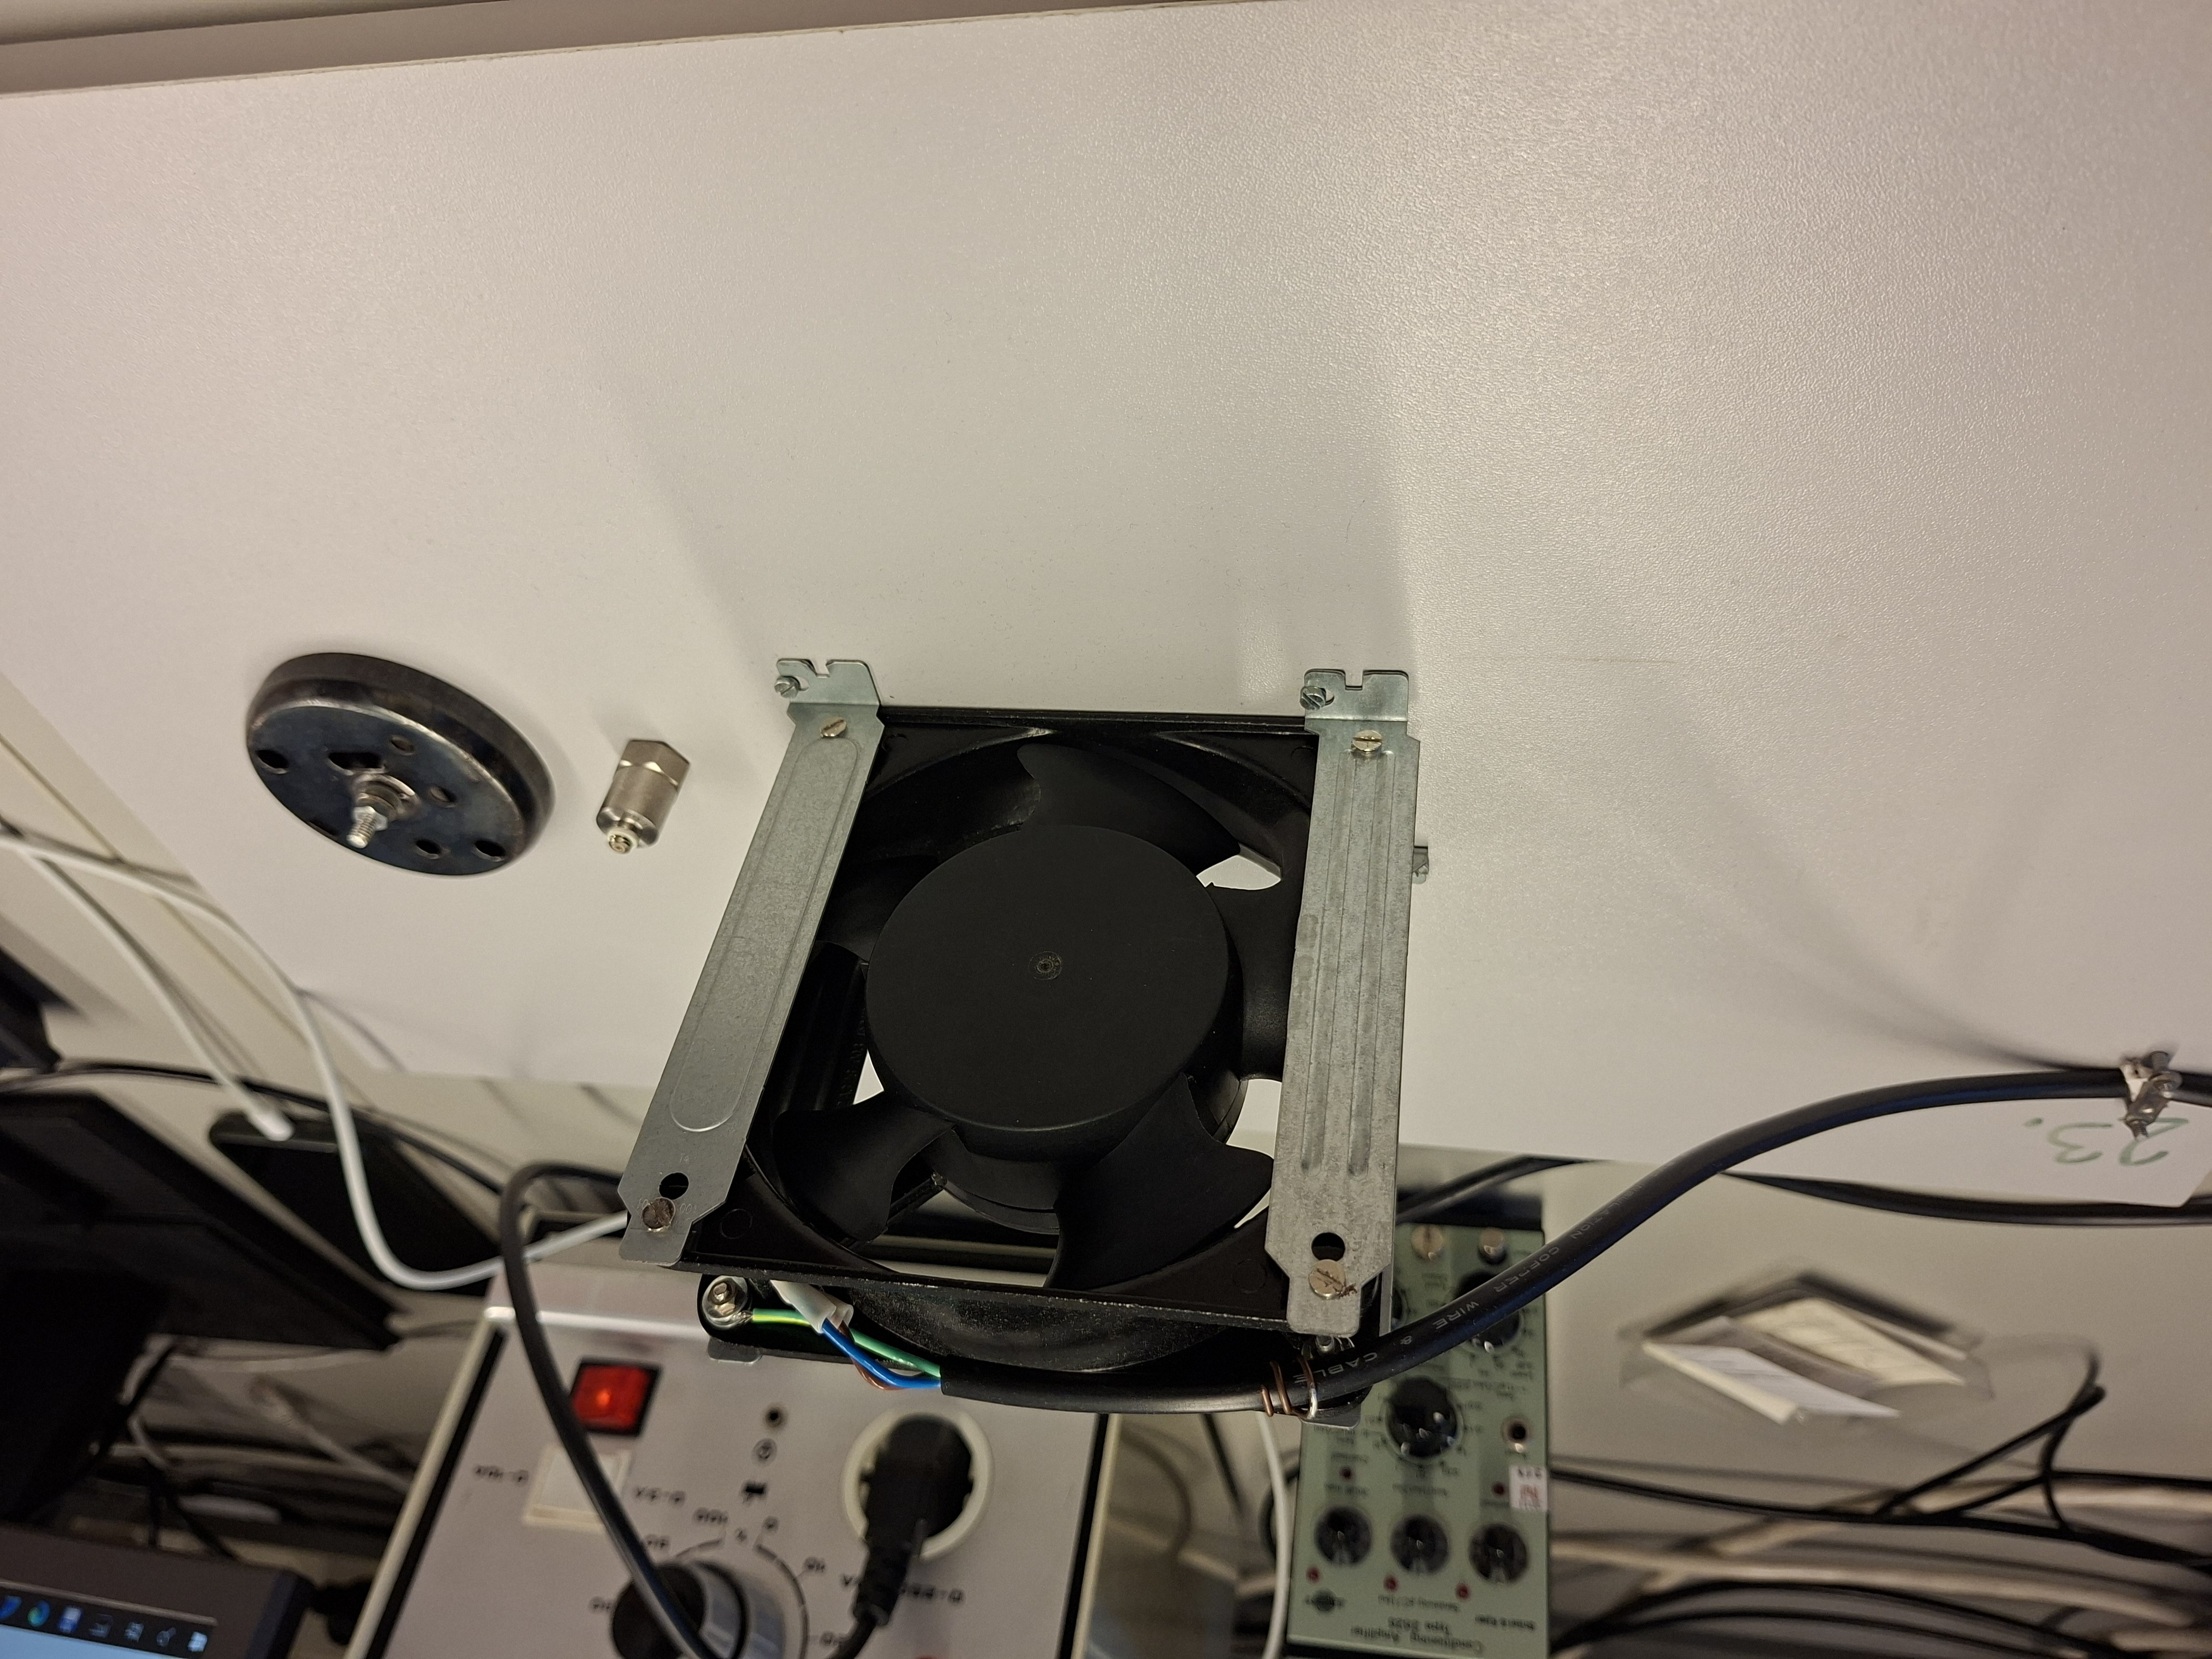
\includegraphics[width = 300px, angle = 180]{../../Kepek/20260914_142213.jpg}	
	\caption{A mérési elrendezés.}
	\label{fig:meresi-elrendezes}
\end{figure}

\newpage
Az erősítőt a piezoelektromos rezgésmérő leírása alapján (\abrara{fig:erosito-leiras}) a megfelelő értékűre állítottuk (\abrara{fig:erosito-beallitas}), majd a ventillátorról leolvasva (\abrara{fig:ventillator_hatulja}) annak névleges feszültségét, üzembe helyeztük 230 [V]-ot ráadva.


\begin{figure}[H]
	\centering
	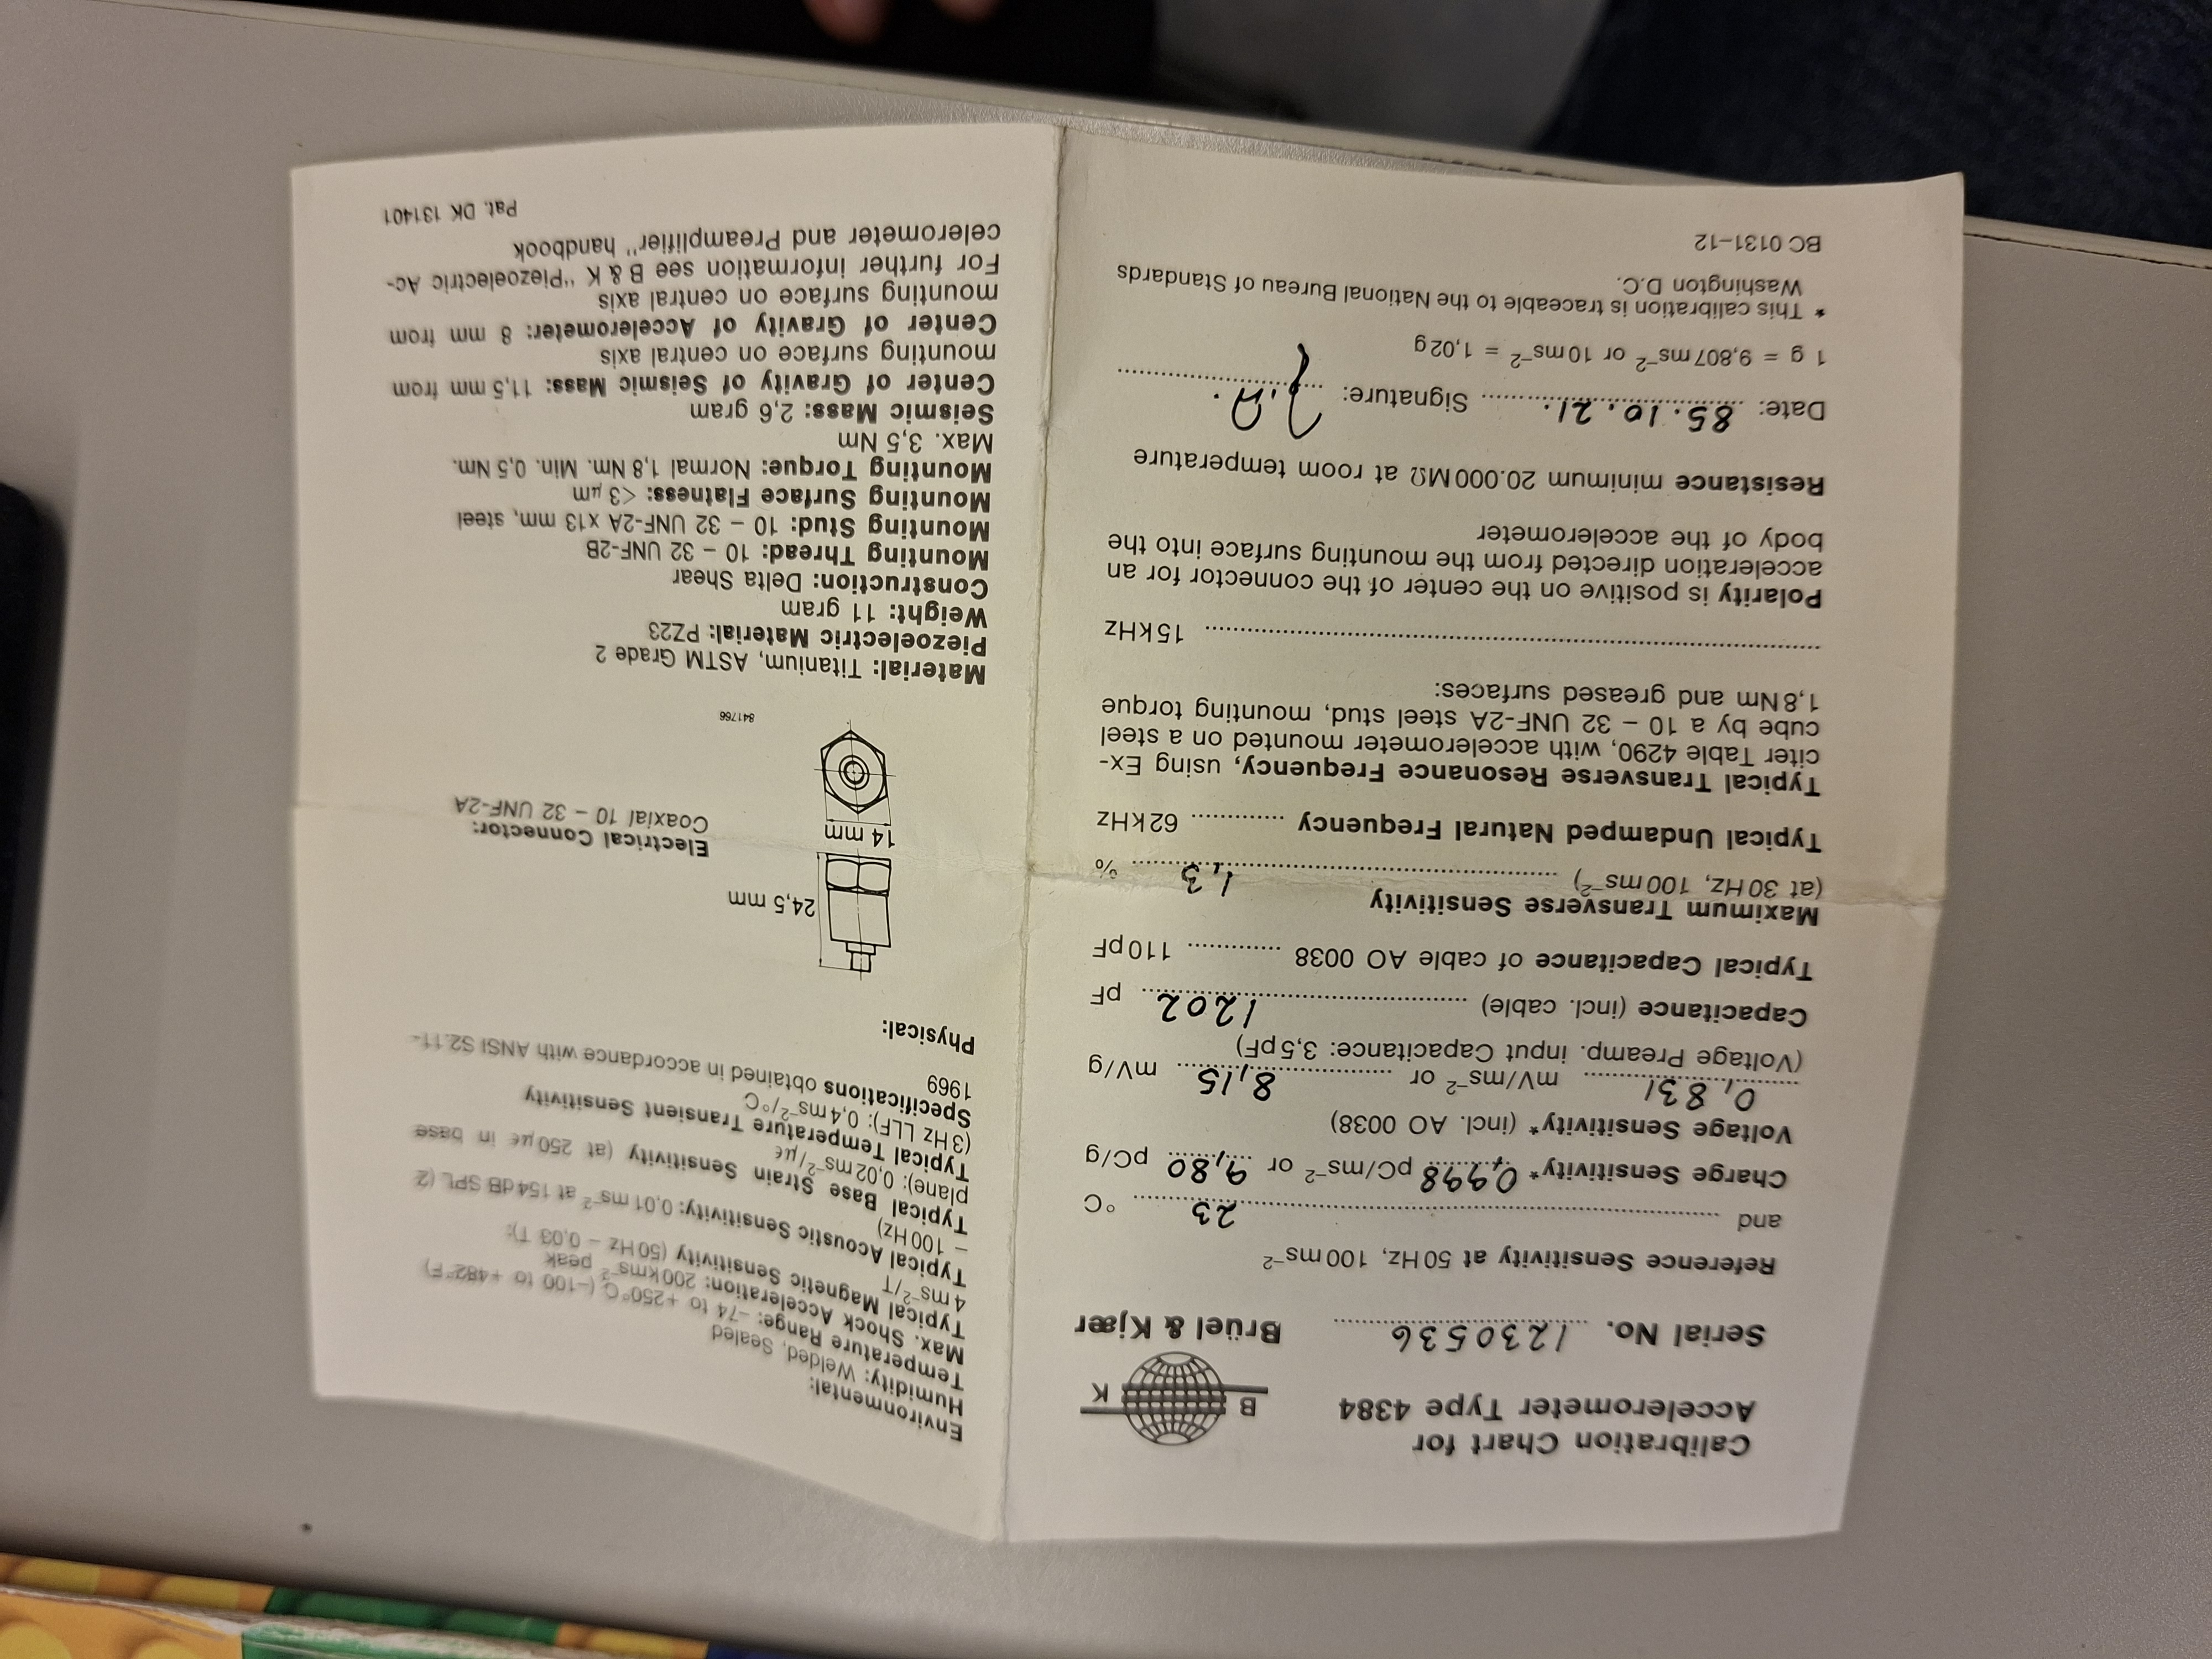
\includegraphics[width = 300px, angle = 180]{../../Kepek/20260914_142447.jpg}	
	\caption{A beállított erősítő.}
	\label{fig:erosito-leiras}
\end{figure}

\begin{figure}[H]
	\centering
	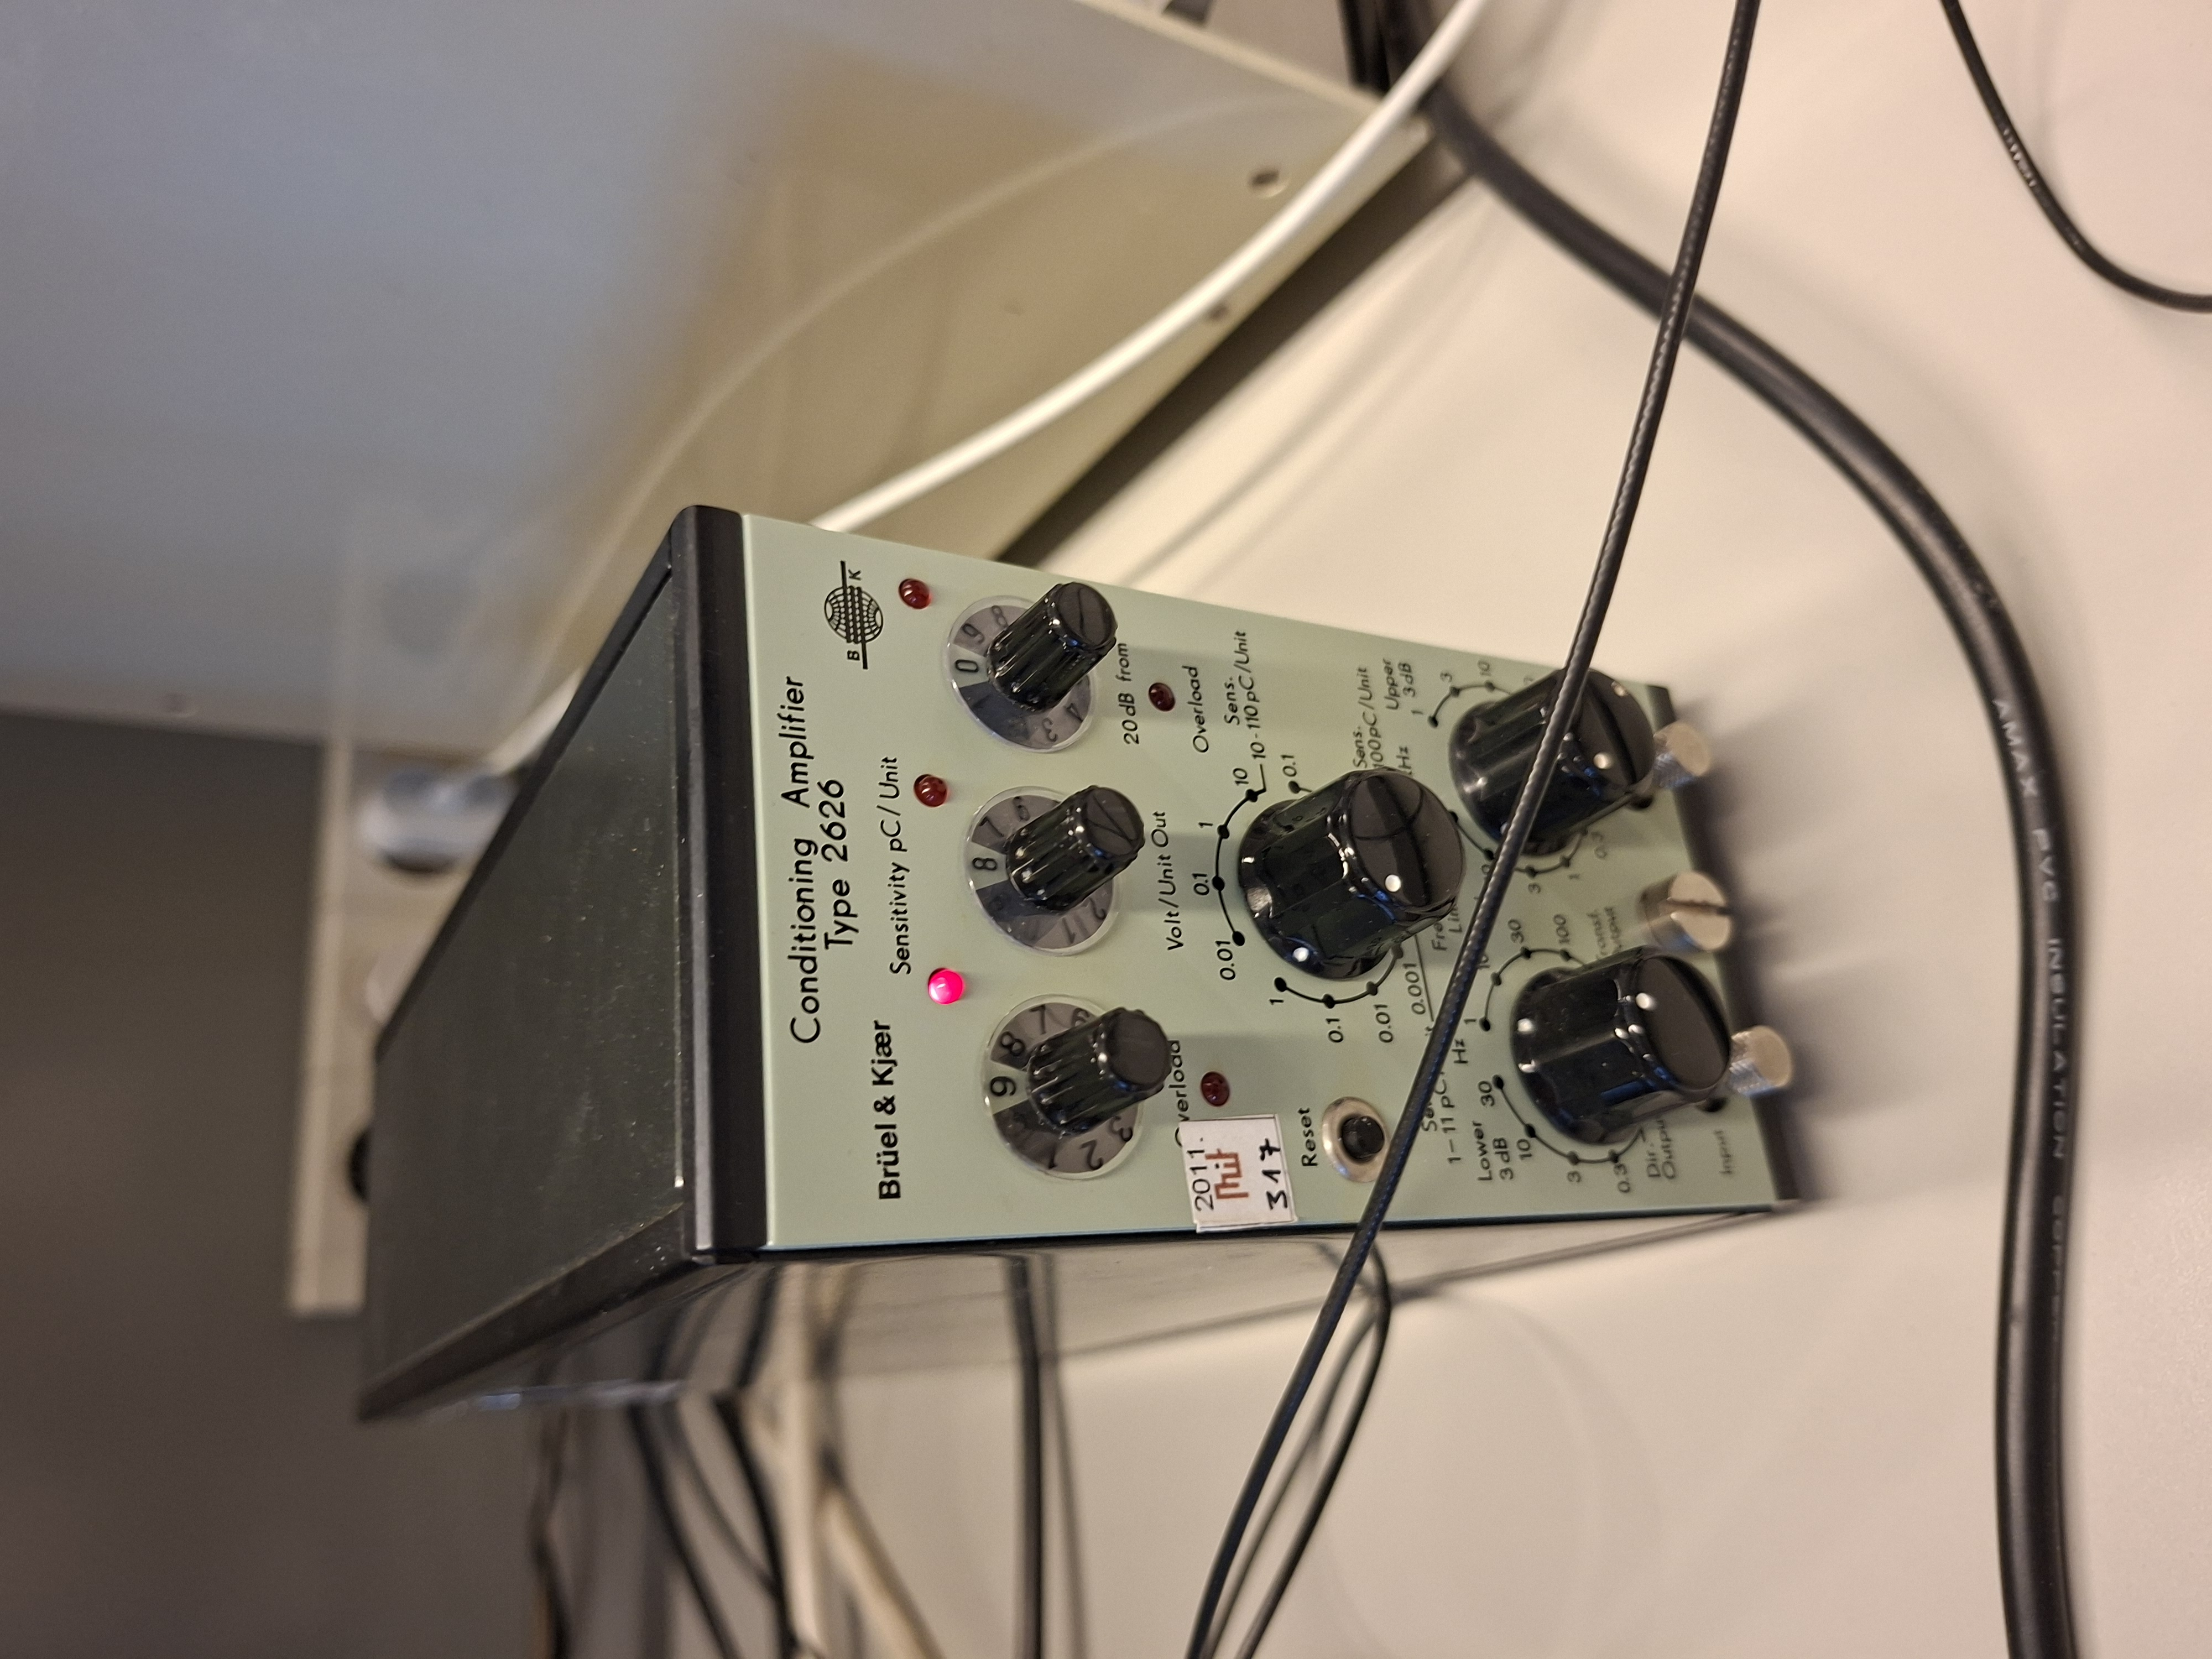
\includegraphics[width = 300px, angle = 270]{../../Kepek/20260914_144113.jpg}	
	\caption{A beállított erősítő.}
	\label{fig:erosito-beallitas}
\end{figure}

\begin{figure}[H]
	\centering
	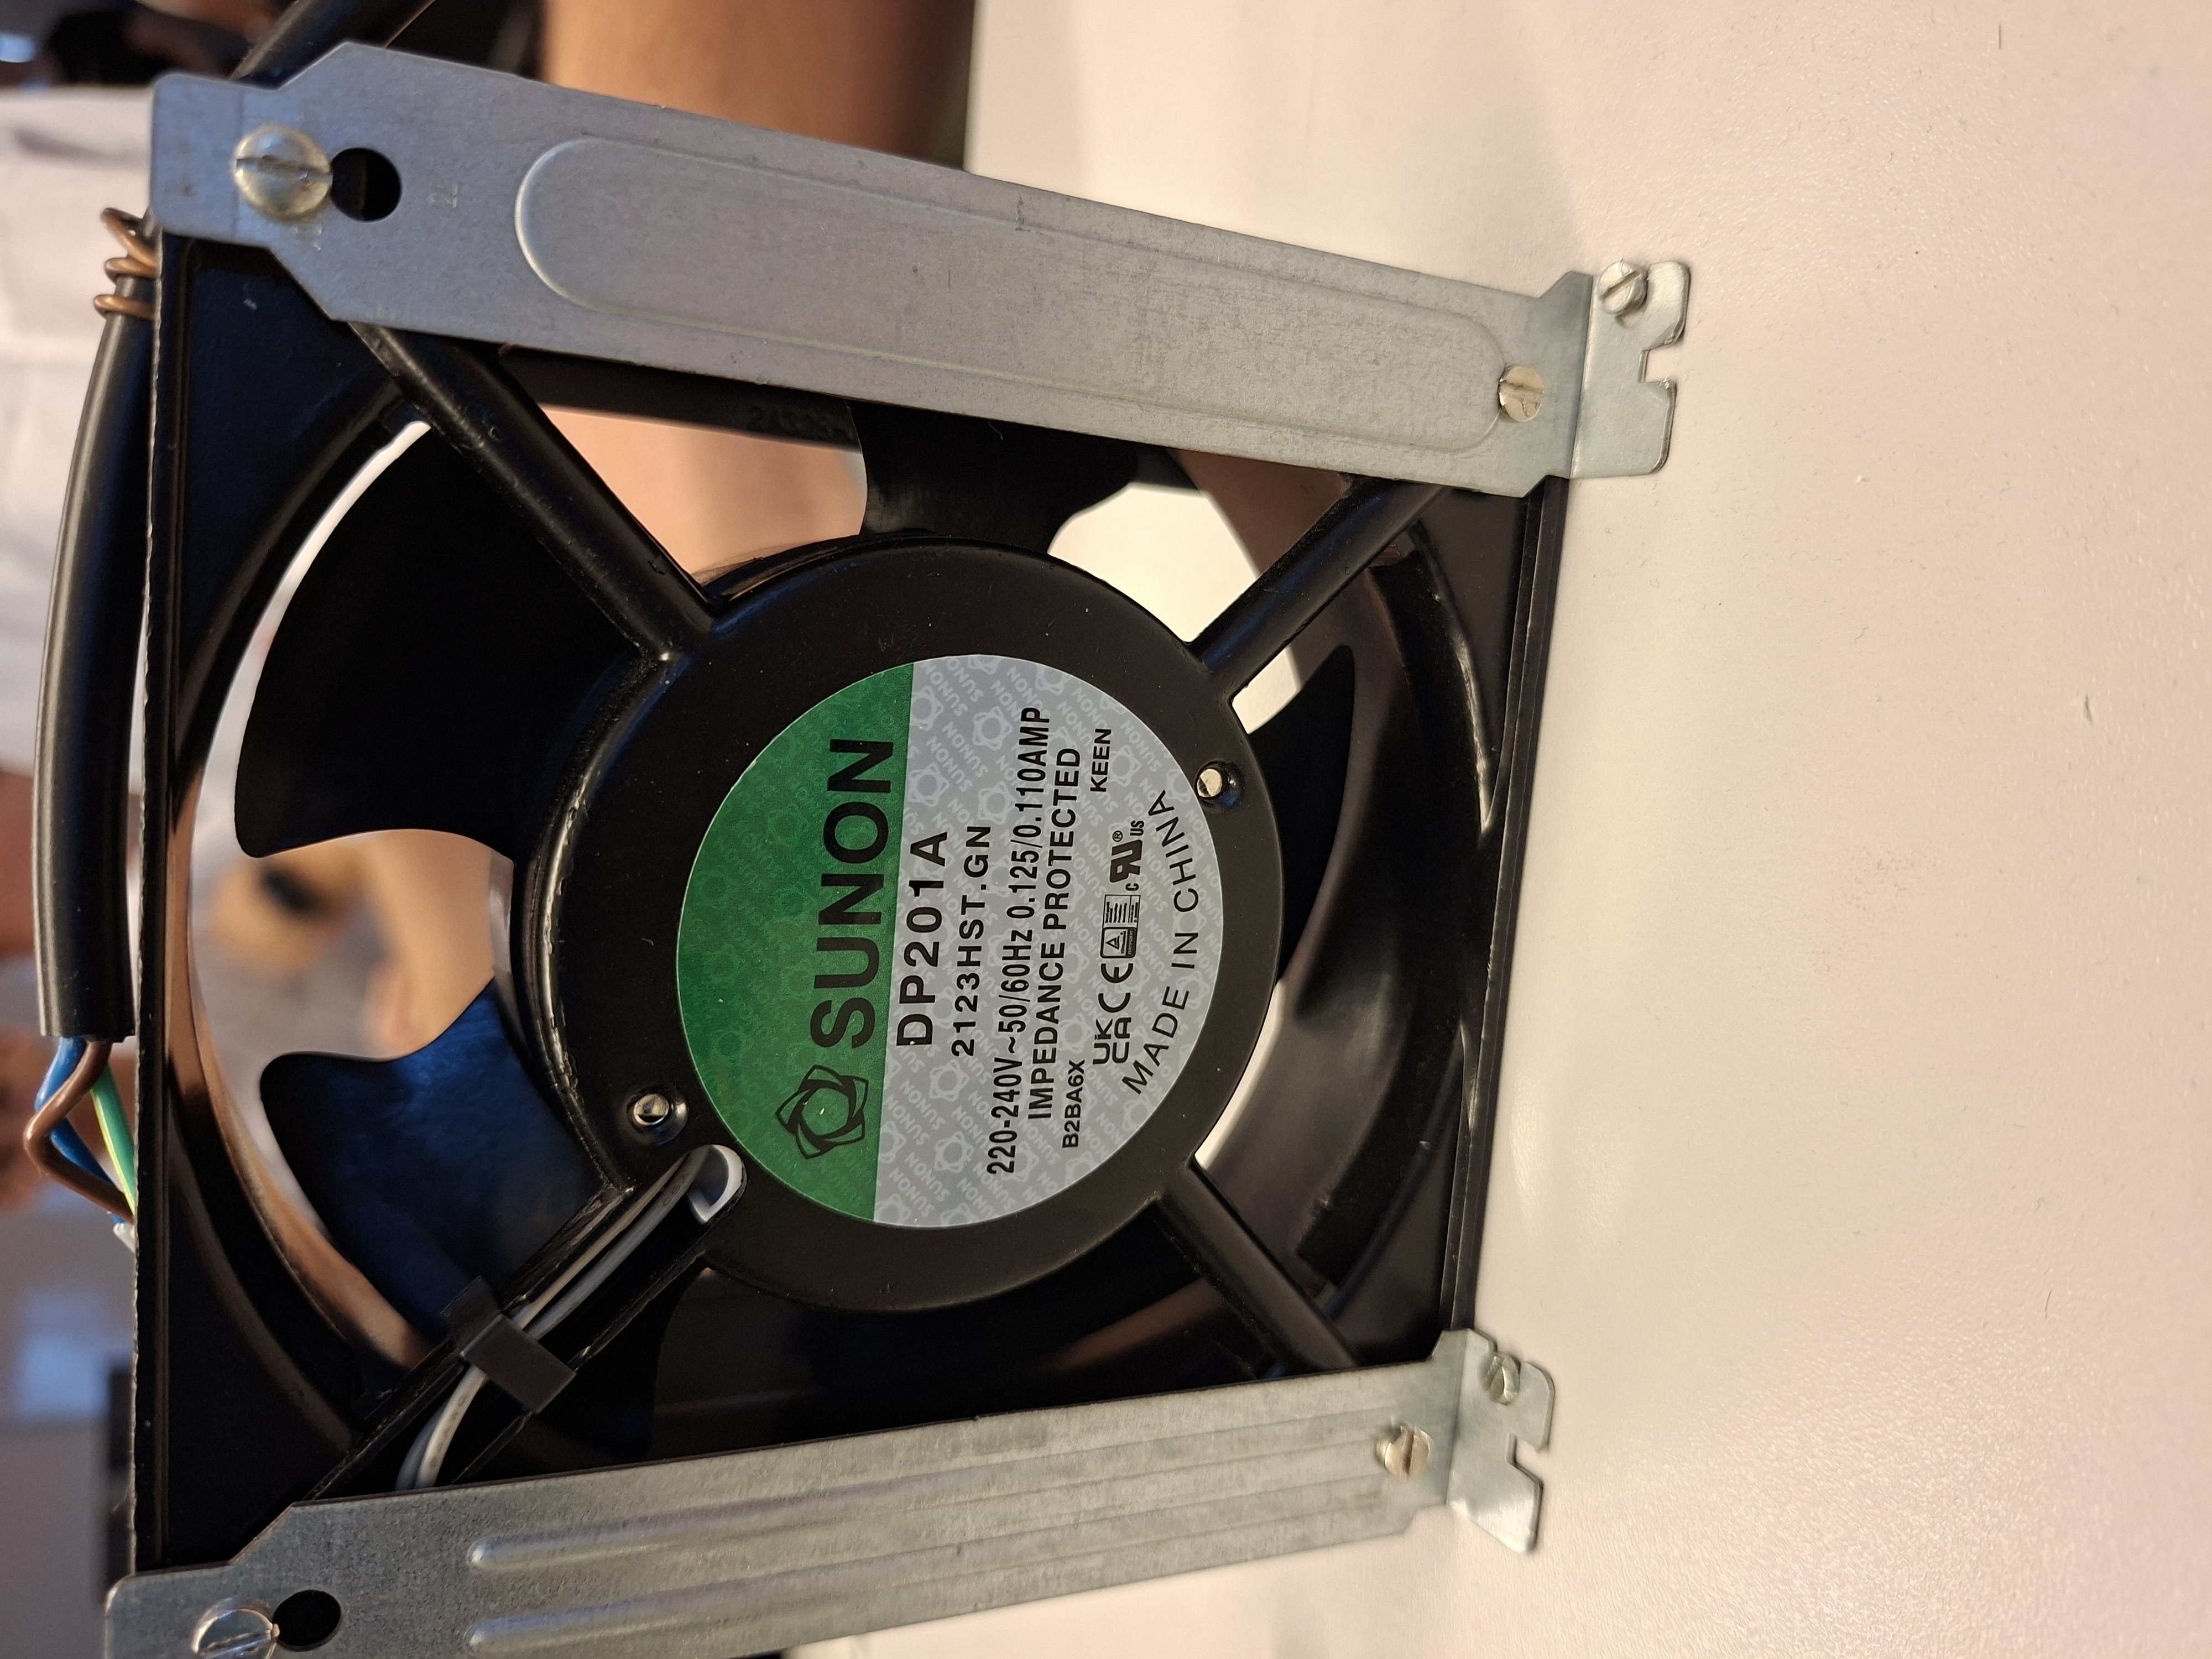
\includegraphics[width = 300px, angle = 270]{../../Kepek/20260914_142201.jpg}	
	\caption{A beállított erősítő.}
	\label{fig:ventillator_hatulja}
\end{figure}


Az Audacity program segítségével egy felvételt készítettünk ezen a feszültségen, majd a felvételt mentettük. A rögzített felvételt Matlabba betöltve tudtuk elemezni, erre az \texttt{audioread} függvényt használtuk.\\

Első lépésként a jel időben változó frekvenciatartalmát vizsgáltuk, a \texttt{spectogram} függvény segítségével. Ebből le tudtuk olvasni a legmagasabb mérendő frekvencia komponenst, amely alapján az ideális mintavételi frekvencia is meghatározható.\\

Ahogy a(z) \abrara{fig:meres1-spektrogram} szemlélteti, $f_{max}$ értéke $0,85$ [kHz] körül található, és a Nyquist-tétel alapján az ideális mintavételi frekvencia $f_s > 2 \cdot f_{max} = 1,7$  [kHz]. Így megállapítható, hogy a mintavételi frekvenciát már biztosan elegendő lenne 2 [kHz] környékére állítani, de az esetlegesen megjelenő magasabb frekvenciakomponensek detektálása érdekében a következő mérések során, 44100 [Hz]-es mintatvételi frekvenciát használtunk továbbra is.

\begin{figure}[H]
\centering
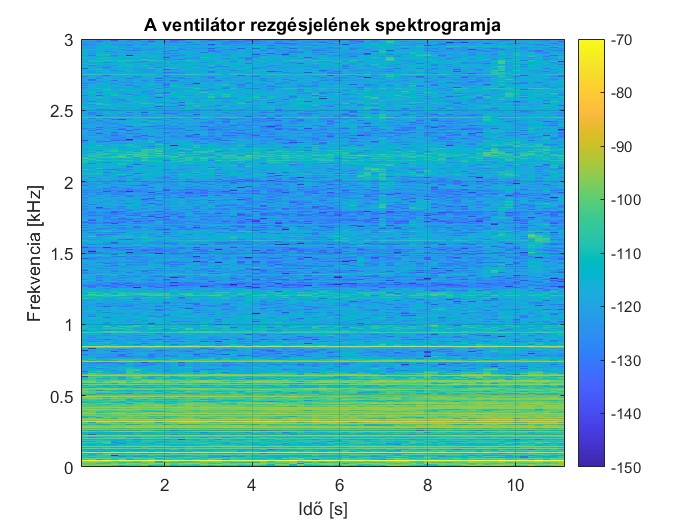
\includegraphics[width=\textwidth]{../../Kepek/Spektogram.jpg}
\caption{A ventilátor rezgésjelének spektrogramja.}
\label{fig:meres1-spektrogram}
\end{figure}
\par

A mért jelet ezt követően a töltéserősítő erősítésével és az érzékelő kalibrációs adataival gyorsulásértékké számítottuk át a következő folyamatábrát figyelembe véve a jel alakulásáról:


\begin{figure}[H]
\centering
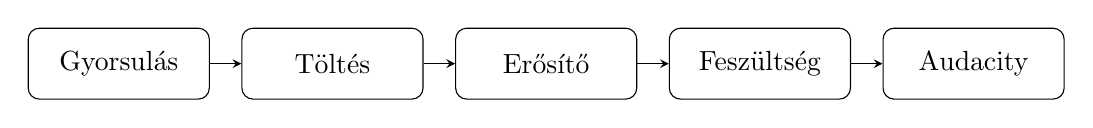
\begin{tikzpicture}[node distance=0.4cm, >=stealth]
	\node[draw, rounded corners, minimum width=2.3cm, minimum height=0.9cm] (gyorsulas) {Gyorsulás};
	\node[draw, rounded corners, minimum width=2.3cm, minimum height=0.9cm, right=0.4cm of gyorsulas] (toltes) {Töltés};
	\node[draw, rounded corners, minimum width=2.3cm, minimum height=0.9cm, right=0.4cm of toltes] (erosito) {Erősítő};
	\node[draw, rounded corners, minimum width=2.3cm, minimum height=0.9cm, right=0.4cm of erosito] (feszultseg) {Feszültség};
	\node[draw, rounded corners, minimum width=2.3cm, minimum height=0.9cm, right=0.4cm of feszultseg] (audacity) {Audacity};
	\draw[->] (gyorsulas) -- (toltes);
	\draw[->] (toltes) -- (erosito);
	\draw[->] (erosito) -- (feszultseg);
	\draw[->] (feszultseg) -- (audacity);
\end{tikzpicture}
\caption{A jel útja a gyorsulásérzékelőtől a feszültségjelig.}
\label{fig:meres1-folyamatabra}
\end{figure}


\begin{equation}
a[n] = \frac{x[n]}{0{,}1 \cdot 0{,}998} \cdot \frac{0{,}04}{0{,}0054},
\label{eq:meres1-acc}
\end{equation}

ahol $x[n]$ a beolvasott mérési jel, $a[n]$ pedig az átszámított gyorsulásjel.  A konstans értékeket a következő képpen származtattuk: a töltéserősítő erősítése $0{,}1$ [V/Unit out], az érzékelő kalibrációs adata $0{,}998$ [pC/ms-2], az oszcilloszkóp peak-to-peak értéke $0{,}04$ [V], az audacityben rögzített jel peak-to-peak értéke $0{,}0054$ [-]. Az így kapott gyorsulásértékeket a(z) \abrara{fig:meres1-gyorsulas} szemlélteti\\

\begin{figure}[H]
\centering
\includegraphics[width=\textwidth]{../../Kepek/Rezgesjel_ms2.jpg}
\caption{A rezgésjel nagysága.}
\label{fig:meres1-gyorsulas}
\end{figure}

\newpage

\feladat{2}

\subsubsection*{Feladat rövid megfogalmazása}

A toroid transzformátor kimenő feszültségének változtatásával változtassa a fordulatszámot, és készítsen több felvételt is! Azonosítsa a 0..500 Hz tartományban detektálható komponenseket! Határozza meg az aszinkron motor slipjét névleges feszültségen! Ügyeljen a DFT pontszámának megválasztására!

\subsubsection*{Feladat megoldása}
A második feladat során a mérést a ventillátor bekapcsolása előtt indítottuk, majd a toroid transzformátor kimenő feszültségének változtatásával a ventilátor névléges feszültségre kapcsoltuk, és végül a feszültséget ismét 0 Voltra kapcsoltuk.
\newpage

A mérés során szintén a \texttt{spectogram} függvény segítségével olvastuk le a 0..500 Hz tartományba detektálható komponenseket.\\

\begin{figure}[H]
\centering
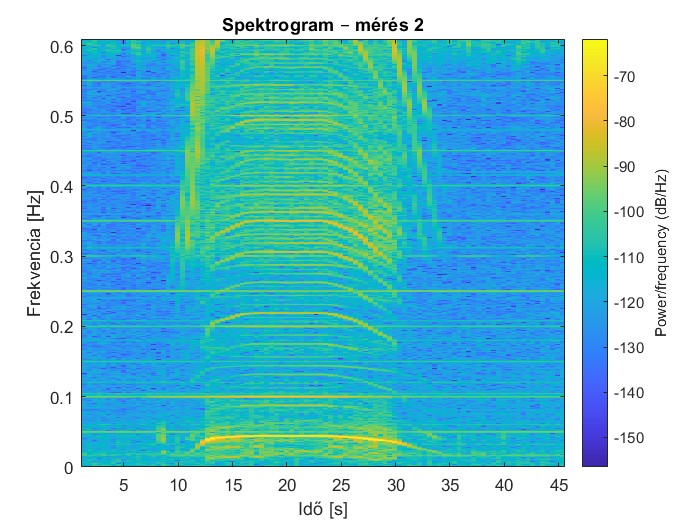
\includegraphics[width=\textwidth]{../../Kepek/Spektogram_2.jpg}
\caption{A ventilátor rezgésének spektrogramja}
\label{fig:meres2-Spektogram}
\end{figure}

A spektogramról látható, hogy az 50 Hz-es hálózati frekvencia dominánsan megjelenik konstans értékként. Ezen felül ennek a frekvenciának a felharmónikusai is megjelennekek a spektrumon, a jel nemlineáris torzulásából és a forgó mechanikai rendszer periodikus mozgásából eredően, az 50 Hz többszörösein.

\begin{figure}[H]
\centering
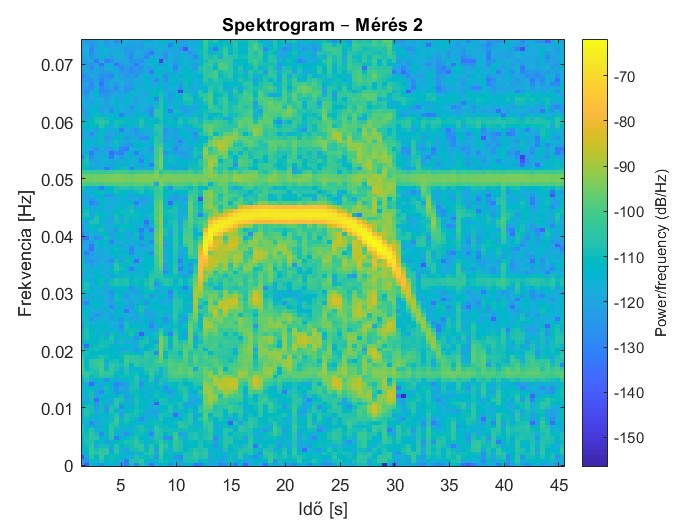
\includegraphics[width=\textwidth]{../../Kepek/Ventillator_frekvenciaja.jpg}
\caption{A ventillátor forgási frekvenciája}
\label{fig:ventillator-frekvencia}
\end{figure}

A 4. ábrán megfigyelhető, hogy a ventilátor működésének domináns frekvenciakomponense körülbelül $43{,}74\,\mathrm{Hz}$ érték körül helyezkedik el. Ennek és az ismert hálózati frekvencia ($50\,\mathrm{Hz}$) ismeretének a segítségével ki tudtuk számítani a ventillátor slipjét az alábbi képlet segítségével:

\begin{equation}
	\text{Slip} = \frac{f_{\text{hálózat}} - f_{\text{ventilátor}}}{f_{\text{hálózat}}} \cdot 100\%
\end{equation}

Behelyettesítve:

\begin{equation}
	\text{Slip} = \frac{50 - 43{,}74}{50} \cdot 100\% \approx 12{,}52\%
\end{equation}

%Moduláció?



\feladat{3}

\subsubsection*{Feladat rövid megfogalmazása}

Helyezze el a rezgésérzékelőt a doboz oldalán, és vezessen változó frekvenciájú szinuszos jelet a hangsugárzóra! Az „L” alakú lemez beállításával érje el, hogy bizonyos frekvenciákon „megzörgesse” a lemezt. A zörgés jelenségét mellőzve mérje meg a bemeneti feszültség és a gyorsulásjel közötti amplitúdómenetet! Ehhez MATLAB-ban generáljon megfelelő időtartamú fehérzajt! Értelmezze a végeredményt, indokolja meg a fontosabb töréspontokat, maximum- és minimumhelyeket!

\subsubsection*{Feladat megoldása}
\Pointilles{10}

\feladat{4}

\subsubsection*{Feladat rövid megfogalmazása}

Milyen gerjesztést és analízist alkalmazna, amellyel észlelhető, ha az „L” alakú lemez túl közel kerül a dobozhoz, azaz káros mechanikai jelenség lép fel? A mérés során csak a „megfelelő” és a „nem megfelelő” állapot megkülönböztetésére alkalmas mérési módszert kell kidolgozni és demonstrálni, az állapot automatikus felismerése nem feladat.

\subsubsection*{Feladat megoldása}
\Pointilles{10}

\feladat{5}

\subsubsection*{Feladat rövid megfogalmazása}

\textit{(kiegészítő mérési feladat)} Gyorsulásérzékelőt használva rögzítse a megütött csengőhangját! Határozza meg a főbb komponenseket, és azok lecsengésének időállandóját!

\subsubsection*{Feladat megoldása}
A mérés során az alábbi x.ábrán látható módon helyeztük el a gyorsulásérzékelőt a csengő mellé, majd a csengőt megütve rögzítettük annak a lecsengését. A rögzített felvételt a korábbi feladatokban leírt módon feldolgoztuk, majd a spektogramját vizsgáltuk, ami az alábbi x. ábrán látható.

%\begin{figure}[H] ezt majd tedd be
%\centering
%\includegraphics[width=\textwidth]{Rezgesjel_ms2.jpg}
%\caption{Mérési összeállítás}
%\label{fig:meres-osszeallitas}
%\end{figure}

\begin{figure}[H]
\centering
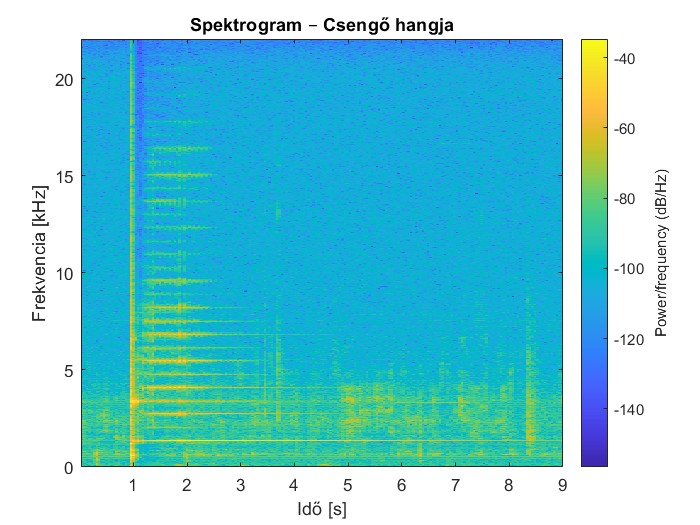
\includegraphics[width=\textwidth]{../../Kepek/Csengo_hangja.jpg}
\caption{A csengő hangjának spektogramja.}
\label{fig:csengo-hangja}
\end{figure}

A spektogramról leolvashatóak a főbb komponensei a csengésnek, illetve ezeknek az időállandói is meghatározhatóak. Az időállandók leolvasásához megnéztük a csengő megütésnek pillanatában az adott frekvenciasáv intenzitását az oldalsó színskála alapján, majd megkerestük azt az értéket ahol a színskála körülbelül 9 dB-lel halványabb értéket mutatott. A csengő hangjának mesterséges előállításához az alábbi frekvenciákat használtuk fel, a hozzájuk választott időállandókkal:
\newpage

\begin{itemize}
	\item $1400\,\mathrm{Hz}$, $\tau = 3.5\,\mathrm{s}$
	\item $3400\,\mathrm{Hz}$, $\tau = 1.2\,\mathrm{s}$
	\item $5600\,\mathrm{Hz}$, $\tau = 0.6\,\mathrm{s}$
	\item $6900\,\mathrm{Hz}$, $\tau = 0.4\,\mathrm{s}$
\end{itemize}


\feladat{6}

\subsubsection*{Feladat rövid megfogalmazása}

\textit{(kiegészítő mérési feladat)} Az előző feladat eredményeinek felhasználásával generáljon „csengőhangot”! A jelet hallgassa meg hangszórón, és értékelje az eredményt!

\subsubsection*{Feladat megoldása}
A csengőhang rekonstruálása során a négy domináns frekvenciához exponenciálisan lecsengő szinuszos kompnenseket hoztunk létre, az alábbi összefüggés szerint:

\begin{equation}
	x(t)_i = A_i \cdot e^{-\frac{t}{\tau_i}} \cdot \sin(2\pi f_i t)
\end{equation}

Az egyes részhangokat szuperpozícióval összegeztük egy közös kimeneti vektorban. Mivel a komponensek összeadódása miatt a hullámforma amplitúdója meghaladhatja az egységet, a kód végén csúcsértékre történő normalizálást hajtottunk végre, elkerülve az audiolejátszás során fellépő túlvezérlést.

A rekonstruált csengőhang spektogramja az alábbi x. ábrán látható.

\begin{figure}[H]
\centering
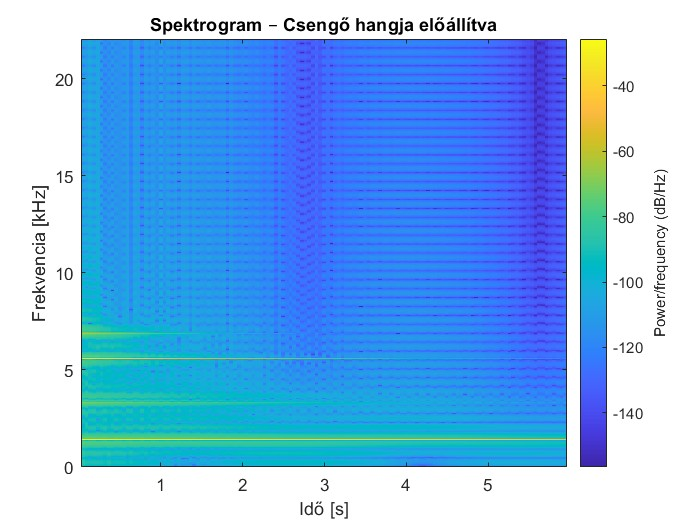
\includegraphics[width=\textwidth]{../../Kepek/Csengo_hangja_eloallitva.jpg}
\caption{A csengő általunk előállított hangjának spektogramja.}
\label{fig:csengo-hangja_mestersges}
\end{figure}

Az előállított hangot a MATLAB \texttt{sound} függvényével hallgattuk meg, és a hangzás alapján megállapítható, hogy a csengőhangot sikerült megfelelően rekonstruálni.

\section*{Függelék}
\subsection*{MATLAB kódok}

\lstinputlisting[
    caption={Az első mérés MATLAB-kódja},
    label={lst:meres1-matlab}
]{../../MATLAB/meres1.m}


\end{document}
